%\documentclass[twocolumn]{article}
\documentclass[./exercises.tex]{subfiles}
\begin{document}

\section{Den kosmiska distansstegen -Inledning}
Ingen enskild metod finns för att uppskatta samtliga avstånd i univsersum utan för att mäta
upp avstånd till astronomiska objekt allt längre och längre bort så används olika metoder
som kalibreras med hjälp av metoder som används för kortare avstånd.
Detta är anledningen till uttrycket ``stege'' eftersom metoder för längre avstånd är beroende
av metoder för kortare avstånd då längre avståndsmätningsmetoderna (stegpinne ovanför) kalibreras  mot avstånd
uppmätt med metoder för att mäta kortare avstånd (stegpinne nedanför).

\begin{figure}[H]
  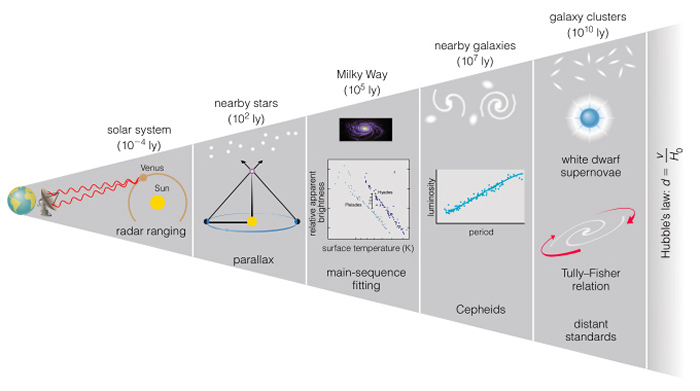
\includegraphics[width=\linewidth]{distance_ladder.jpg}
  \caption{Avståndsstegen}
  \label{fig4}
\end{figure}

 Exempelvis så kan man använda radar för att mäta upp avstånd till
planeter och få ett exakt avstånd till solen, detta kan sägas vara den första stegpinnen om vi bortser
från tidgare astronomers beräkningar av avstånd med analoga mätmetoder.\\
 Då korrekt avstånd till solen erhållits så blir den dubbla jordbaneradien den s.k. baslinjen (``baseline'') för parallaxmätningar.
Jordbaserade parallaxmätningar är möjliga upp till ca 40 parsec (130 ljusår)\footnote{\url{https://www.atnf.csiro.au/outreach/education/senior/astrophysics/parallaxlimits.html}}.
De bästa landbaserade teleskopmätningarna har ca en hundradels bågssekunds upplösning därefter fås problem
med ljusets genomgång hos atmosfären.\\
Atmosfären sprider och bryter strålarna så att himlakroppar inte kan urskiljas från varandra så
därför har man skickat upp satelliter. \\
%Hipparchos ( HIgh Precision PARallax COllecting Satellite, 1989-1993) med upplösningen 1 millibågsekund varmed
%man identifierade positionerna för ca 100 000 stjärnor där maximala avståndet var flera hundra ljusår bort.
%Gaia (2013- 2025 beräknat) med upplösningen 20 mikro bågsekunder som har hittills mätt avståndet till ca 1 miljard
%astronomiska objekt med noggrannheten ca 10\% för avstånd ca 30 000 (10 000 parsec)ljusår bort.

För att avståndsbestämma stjärnor som ligger längre bort, upp till ca 10 000 pc vilket är den nuvarande gränsen
för rymdbaserade parallaxmätningar (ca 500pc till 10 000 pc beroende på hur stor noggrannhet som krävs) så måste man
ta till statistiska metoder s.k. ``mainsequence fitting'' - anpassning (eng. fitting) till statistiska data.
Denna metod kallas även spektroskopisk parallax trots att den inte har något gemensamt med geometrisk parallaxmätningar.
Ejnar Hertzsprung och Henry Norris Russell fick år 1911 respektive 1913  plottade färgen och den relativa
magnituden till stjärnor som avståndbestämts med parallax metoden. Deras slutsats var att
färgen på stjärnan är en funktion av dess luminositet dvs.dess uteffekt $L$ dvs. den elektromagnetiska strålningseffekt i Watt som
sändes ut av stjärnan.
Korrekt identifiering av färgfördelning av det stjärnansljus som emitteras så korresponderar entydigt till dess uteffekt $L$.
Med kännedom om stjärnans uteffekt/luminositet och den uppmätta effekttätheten watt per kvadratmeter
$F$(på engelska flux) i sensorn här på jorden så mätes avståndet $r$ genom känd radiolänkteori som säger att
den mottagna effekttätheten är omvänt proportionellt mot avståndet i kvadrat men proportionellt mot uteffekten.

Vidare så gör man antagandet att vår del av universum inte skiljer sig nämnvärt från andra delar av 
universom där det finns stjärnor, att det måste gälla att fördelningen av varma och kalla stjärnor måste rimiligtvis 
se ungefär lika ut var man än mäter i universum givet att den volym man betraktar är tillräckligt stor p.g.a. kända statistiska principer.

Därför kallar man fördelningen av varma och kalla stjärnor i ett Hertzsprung-Russel diagram
 ``main sequence''. Att antagandet är förmodligen är rimligt torde bygga på det faktum att de kemiska processerna 
som avgör en stjärnas temperatur och därmed dess uteffekt måste vara lika överallt i universum eftersom det inte borde kunna finnas
andra naturlagar i andra delar av unviersum.\\

Med kännedom alltså endast av färgen så erhålles uteffekten och avståndet kan beräknas. Fördelningen av varma och kalla stjärnor i ``main sequence''
dvs. dess grafiska utseende tjänar såsom kontrollfördelning när man avståndsbestämmer en hop av stjärnor dvs. man
bör inte använda  ``main sequence'' för att avståndsbestämma stjärnor i ett kluster som inte följer fördelningen
så när så hur pass bra en given fördelning mappar mot ``main sequence'' blir då en kvalitetsparameter på
avståndsmätningarna\\ 

För att bestämma längre avstånd t.o.m. till andra galaxer så används närmast s.k. Cepheid varibaler. Henrietta Swan Leavitt upptäckte 1908 att de tusentals variabla stjärnor i magellanska molnen
har en periodicitet i sin luminans som är en funktion av luminansens toppvärde. Med kännedom
av tidigare parallax-mätningar så kunde man därför bestämma de uteffekter som är unikt relaterade
till stjärnans periodtid. Sådana typer av stjärnor kallades Cepheidvariabler därför att de första variabla stjärnan som hittades
var Delta Cephei\footnote{\url{https://en.wikipedia.org/wiki/Delta_Cephei}}.
Hittar man en Cepheidvariabel i  någon annan stjärnhop så mätes periodtiden
för dess svängning som unikt identfierar dess topp-uteffekt $L$ och givet den effekttäthet $F$ som uppmätes
i sensorn så kan avståndet beräknas med radiolänksambandet.
Det faktum att periodtiden unikt identifiera uteffekten torde vara mycket rimligt då en oscillerande
kemisk process med samma periodtid måste rimligtvis vara väldigt unik.

Processer som ger astronomen kännedom om den faktiska uteffekt stjärnan sänder är förståeligen väldig viktigt
och bildar mätnormaler för avståndsmätningar s.k. ``standard candles''. 
Om en ``standard candle'' hittas i ett stjärnklustersom så vet vi avståndet till stjärnklustret därför att 
denna har en entydigt definierad uteffekt.

Cepheidvaribler ger oss avståndsbedöningar upp till ca 30 MParsec (ca 100 miljoner ly)\footnote{\url{https://www.astronomy.ohio-state.edu/ryden.1/ast162_8/notes33.html}} därefter blir de för svåra att detektera.
För att komma ännu längre bort så använder man en speciell supernova Typ 1A såsom mätnormal därför att dessa är betydligt
ljusstarkare.
Typ 1A är väldigt speciell och man gör antagandet att samtliga supernovor av denna typ måste ha samma
uteffekt p.g.a. dess unika fysikaliska process.
Avståndet till en sådan supernova har naturligtvis då kalibrerats mot lägre metoder i avståndsstegen
såsom parallax-mätningar och/eller Cepheid variabler. Supernovor av typ 1A är 100 000 gånger ljusstarkare
än den mest ljusstarka Cepheidvaribalen och medger därför avståndsbedömningar på tusentals Mparsec.

För att mäta till universums ytterkanter, sista steget på avståndsstegen, så använder man Hubbelkonstanten och rödskiftet varmed man kan beräkna
avståndet. Antagandet är här, att eftersom universum expanderar och rummet därför dras ut så kommer
den elektromagnetiska strålningen att tänjas ut och öka i sin våglängd och därför kommer ex. en unik väte
övergång på 656nm att förskjutas till allt längre och längre våglängder ju längre bort en stjärna befinner sig därför
att om stjärnan är långt bort så har ljuset tagit förhållandevis längre tid på sig att ta sig hit och ju längre
tid som det har tagit desto längre tid har universum haft på sig att expandera och ju längre universum
har expanderat desto mer har rummet dragits ut och ju mer rummet har dragits ut desto mer har våglängen
som exemplevis började såsom en 656 nm övergång dragit ut.
Hubbelkonstanten har kalibrerats mot lägre nivåer i avståndsstegen såsom Cepheid variabler.

Det finns även avståndsbedömning som bygger på s.k. gravitationsvågor men
detta verkar enligt vår uppfattning vara experimentellt och inget som verkar vara en vedertagen arbetsmetod
inom astrometrin. Grundid\'en är dock densamma - mät en parameter, i detta fall gravitationsfältet, för ett astronomiskt
objekt med kända data, i detta fall massan och avståndet och kalibrera mätningen. Använd därefter
mätinstrumentet för att mäta gravitationen från en annan kropp och erhåll avståendet efter att dess massa
har uppskattats. Det astronomiska objektet för vilket kalibreringen gjorts benämns även med gravitationsmätningar ``'standard candle''därför
att denna kommer att utgöra mätnormalen.
Följande bild illustrerar samtliga kända metoder som används för att bestämma utomgalaktiska avstånd vilka
bygger på olika mer eller mindre komplexa metoder att erhålla en ``standard candle'' eller användning av
gravitationsvågor\footnote{\url{https://en.wikipedia.org/wiki/Cosmic_distance_ladder\#Extragalactic_distance_scale}}
\begin{figure}[H]
  \includegraphics[width=\linewidth]{Extragalactic_distance_ladder.JPG}
  \caption{Utomgalaktiska avståndsstegen}
  \label{fig4}
\end{figure}
Denna rapport delar upp avståndsstegen i det längsta möjliga stegen som kalibrering upp till mätningar med Hubbelkonstanten är möjlig.
De intermediära kalibreringsstegen mellan Cepheid varibaler och typ 1 a Supernovae upp till Hubbelkonstanten
bortses ifrån då dessa har uppfattas såsom steg att för att bekräfta teorin samt för att öka noggrannheten
i beräkningar som redan är möjliga att genomföra.

\section{Avstånd inom planetsystemet -första steget}
\subsection{Antiken}
Aristotoles (384-322 f.Kr.) härledde att jorden måste vara klotformad därför att jordens skugga
 på månen under en månförmörkelse alltid är cirkelformad och resonerade att den enda geometriska figuren som alltid åstadkommer detta oavsett årstid
är om jorden är klotformad. Hade jorden varit en skiva resonerade han så skulle man se skuggan av en skiva som är en ellips eller
ett rakt streck vilket aldrig setts. Vidare så konstaterade han att anledningen till att andra stjärnbilder var
synliga i Alexandria Egypten jämfört med Grekland berodde just på att jorden är en sfär och att dess radie
därför inte har oändlig utsträckning.\\

Erathostenes (276-194 f.Kr.) beräknade jordens radie till 40 000 stadier (6800km) vilket har 8\% noggrannhet.
Han visste att det fanns en brunn i Syene i Egypten som under sommarsolståndet den 21 Juni ser
reflektion av solen nere i brunnen och han visste från Aristotoles resonemang att jorden är en sfär.
Avståndet till Alexandria kände han såsom 5000 stadier och då solen stod som högst den 21 Juni mätte han
skuggan från en ljuspinne (gnomon) till $7^\circ$. Mät skuggans längd $b$ vid basen av gnomon med längden/höjden $h$.
Infallsvinkeln $\Phi$ är $arctan(b/h)$ vilket också är vinkeln mellan ljuspinnens fölängning
till jordens mittpunkt och brunnen i Syene\footnote{\url{https://el.wikipedia.org/}}

\begin{figure}[H]
\begin{center}
  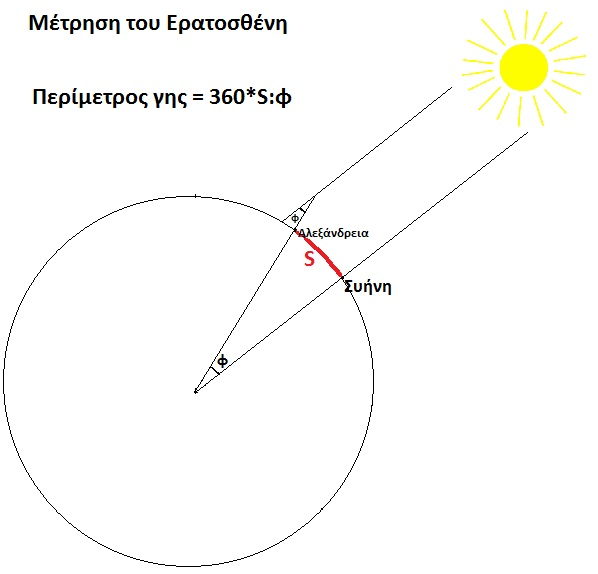
\includegraphics[scale=0.5]{Eratosthenes_measurement.jpg}
  \caption{Eratosthenes mätning}
  \end{center}
  \label{fig4}
\end{figure}

Euklidisk geometri ger att sträckan $S$ (5000 stadier) för håller sig till $7^\circ$ som omkretsen $2\pi r$
förhåller sig till 360 grader.
\begin{flalign*}
\frac{7}{5000}&=\frac{360}{2\pi r}\iff\\
r&=\frac{5000\cdot 360}{2\pi 7}\\
 &=40946 \text{ stadier}
\end{flalign*}
Anledningen till att solens reflektion är synlig i Syenes brunn den 21:a Juni är att den ligger på kräftans vändkrets.\\

Aristotoles resonerade att även månen måste vara sfärsik därför att solljuset på månen bildar en cirkelformad
skugg-gräns som inte skulle finnas om månen endast var en platt cirkel. Om månen var platt så skulle inte heller
månfaserna finnas utan månen skulle då antingen vara fullt upplyst eller inte alls.\footnote{\url{https://youtu.be/kY1gfrhNUIg?t=1530}} \\

Aristarchus (310-230 f.Kr.) beräknade avståndet till månen på följande vis\footnote{\url{https://terrytao.files.wordpress.com/2010/10/cosmic-distance-ladder.pdf}}
\begin{figure}[H]
\begin{center}
  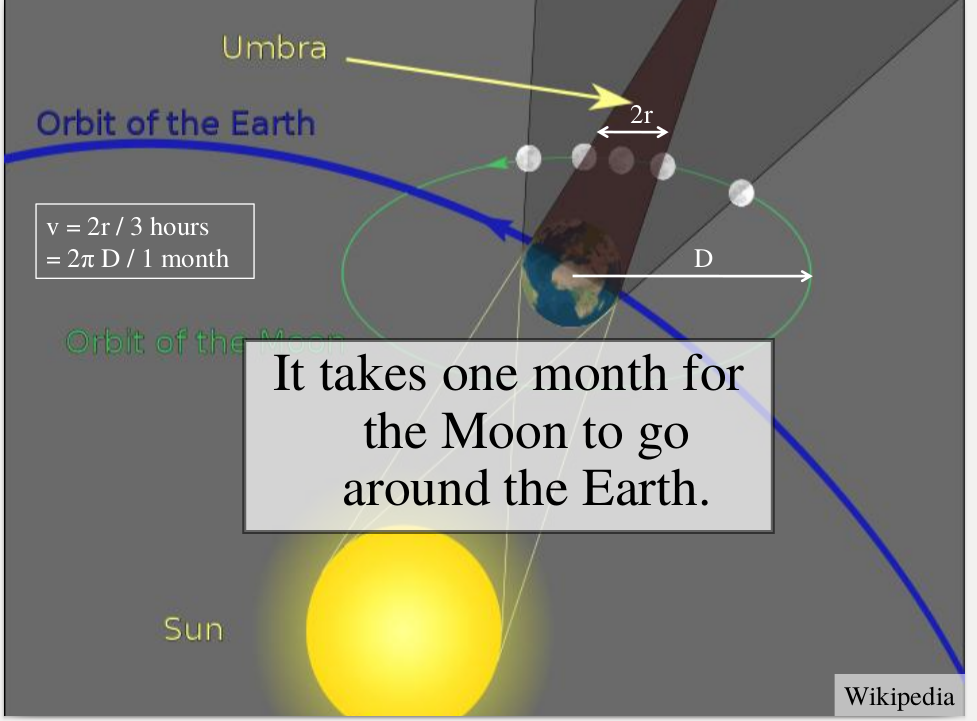
\includegraphics[scale=0.25]{moon_distance.png}
  \caption{Aristarchus beräkning av avståndet till månen}
  \end{center}
  \label{fig4}
\end{figure}
Aristarchus visste att en månförmörkelse varar som längst 3 timmar och att skuggkorridoren som jorden bildar
måste vara ungefär två jordradier $2r$. Då månen tar 28 dagar att komma tillbaka till samma plats så måste gälla
för månens hastighet $v$. Avståndet till månen är radien $R$ av cirkelbanan som månen färdas i.
\begin{flalign*}
v &=\frac{s}{t} =\frac{2r}{3\text{ h}}=\frac{2\pi R}{28\cdot 24 \text{ h}}\iff\\
  R&=\frac{2r\cdot 24\cdot 28}{3\cdot 2\pi}\\ 
   &=71.30141572
\end{flalign*}
Drar man ifrån en jordradie för avståndet till jordytan så fås cirka 70 jordradier.
Aristarchus hade inget värde på $\pi$ utan verkar ha använt närmevärdet 3.7 eller så kompenserade
han för att solen inte är en punktkälla och fick avståndet till månen såsom 60 jordradier vilket också
är det nutida medelavståndet till månen.

På liknande sätt beräknade han månens radie som funktion av avståndet till månen. Han visste att
det tar månen ca 2 minuter att försvinna bortom horisonten
\begin{figure}[H]
\begin{center}
  \includegraphics[scale=0.25]{Moon_distance.png}
  \caption{Aristarchus beräkning av avståndet till månen}
  \end{center}
  \label{fig4}
\end{figure}
För att kunna räkna så verkar Aristarchus ha gjort approximationen att månen inte rör sig nämnvärtmycket
i sin bana under ett dygn. En stråle som är en tangent till jorden representerar siktlinjen från jordens horisont och den sveper 360 grader under
24 timmar.
Om strålen är $D=60$ jordradier lång dvs. avståndet till månen så sveper strålens spets genom hela månbanan
under 24 timmar och det tar uppenbarligen 2 minuter för spetsen att svepa två månradier.
Periferihastigheten för spetsen är $v$
%

\begin{flalign*}
v &=\frac{s}{t} =\frac{2r_{moon}}{2 \text{min}}=\frac{2\pi D}{24\cdot 60 \text{min}}\iff\\
r_{moon}&=\frac{2\pi D}{24\cdot 60 }\approx \frac{D}{229}\approx \frac{D}{180}\\
\end{flalign*}
Aristarchus hade inget värde på $\pi$ utan måste ha approximerat $\pi \approx 4$ för resultatet
$D/180$ och $D$ hade han tidigare räknat till 60 jordradier vilket gav honom
att månens radie är en tredjedel av jordradien, vilket är ganska nära dagens värde 0.2731.

Avseende avståndet till solen så noterade han att vid en solförmörkesle så täcker månen solen nästan
perfekt och därför så måste enligt likformiga trianglar gälla att solens radie $r_{sun}$ också är en 180-del av avståndet $D_{sun}$till solen
$r_{sun}=D_{sun}/180$. Utan teleskop mätte han att halvmånen infaller 12 timmar tidigare med avseende på
nymånen jämfört tiden från halvmåne till fullmåne vilket gav honom ett felaktigt avstånd till solen.
Aristarchus estimerade vinkeln $\theta$ till $87^\circ$ medan dess verkliga värde är $89^\circ 50'$
\begin{figure}[H]
\begin{center}
  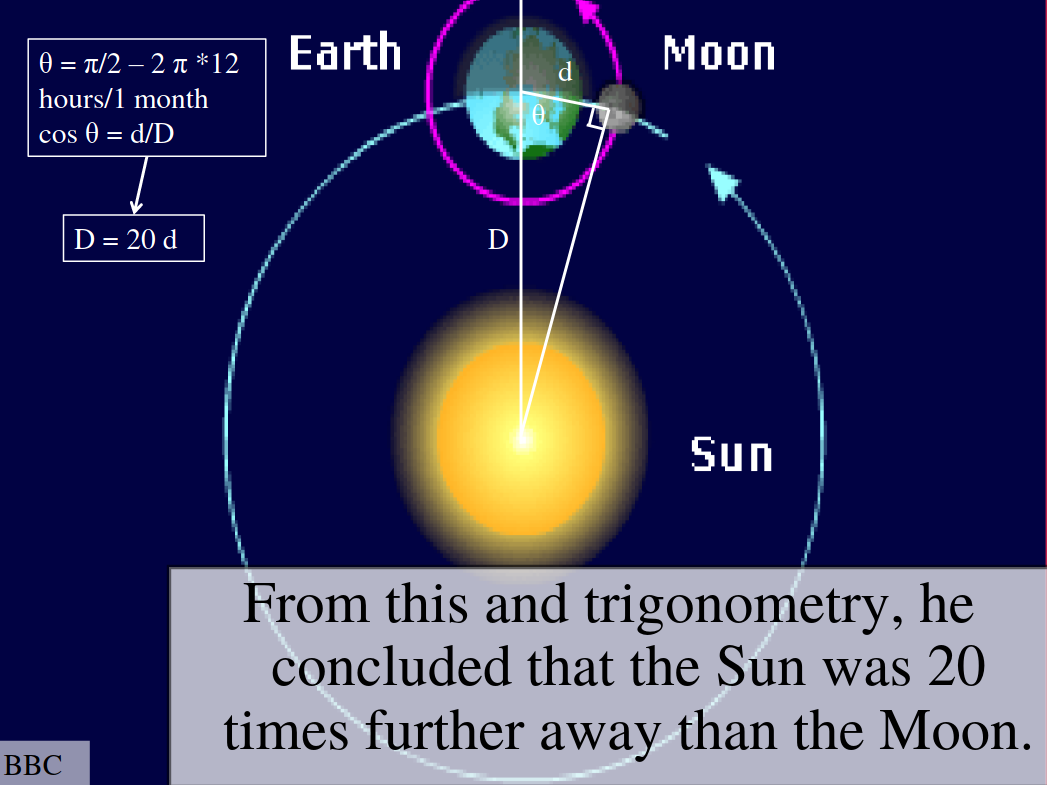
\includegraphics[scale=0.25]{Sun_distance.png}
  \caption{Aristarchus beräkning av avståndet till solen}
  \end{center}
  \label{fig4}
\end{figure}
Det korrekta avståndet till solen är inte 20 månavstånd utan 390 månavstånd
Det felaktiga avståndet till solen gav honom i sin tur ett felaktigt värde på solens storlek
\begin{figure}[H]
\begin{center}
  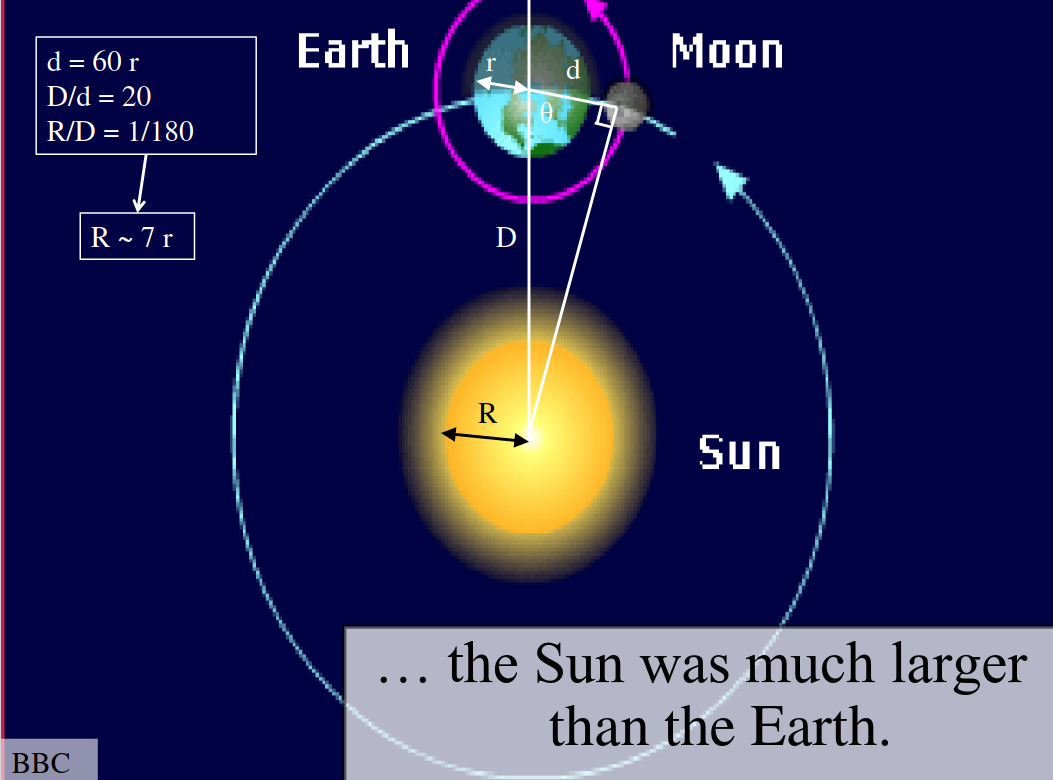
\includegraphics[scale=0.25]{Sun_radius.png}
  \caption{Aristarchus beräkning av solens radie}
  \end{center}
  \label{fig4}
\end{figure}
\begin{flalign*}
d&=60 r\\
\frac{D}{d}&=20\\
\frac{R}{D}&=\frac{1}{180}\iff\\
R&=\frac{D}{180}=\frac{20d}{180}=\frac{20\cdot 60r}{180}=\frac{1200r}{180}\\
 &=6.666666667r\approx 7r
\end{flalign*}
Det korrekta värdet är $\approx 109r$ men det faktum att solen var större än jorden fick
honom att dra slutsatsen att det är jorden som roterar runt solen och inte tvärtom.

\subsection{Copernicus, Tycho Brahe, Kepler och Cook}
Se \url{https://www.youtube.com/watch?v=kY1gfrhNUIg} och \url{https://terrytao.files.wordpress.com/2010/10/cosmic-distance-ladder.pdf}
varifrån också materialet om antiken är lånat.

\subsection{Radarastronomi}

Med hjälp av radar kan man mäta avståndet till Månen, Merkurius, Venus, Mars, Jupiter och Saturnus och sondera dess ytstruktur.
Med de uteffekter som är tillgängliga från Klystroner och Vandringvågrör så kan man typiskt detektera
radareko på 8-10 au avstånd om radarmålytan är 1 km i diameter\footnote{\url{https://en.wikipedia.org/wiki/Radar_astronomy}}. Vidare så är det fördelaktigt att
använda radar för att tracka metorskurar som inte är tillräckligt ljusstarka för att kunna observera med teleskop.
Just nu finns en planetradar tillgänglig i Californien som är Goldstone

 \begin{figure}[H]
\begin{center}
  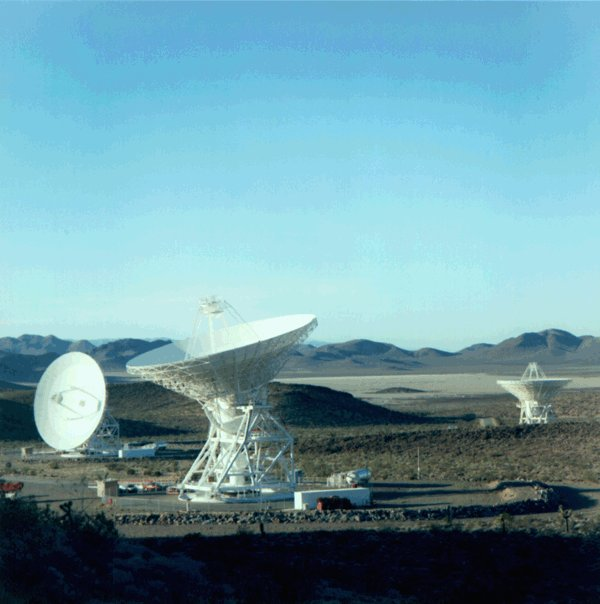
\includegraphics[scale=0.25]{Goldstone_Deep_Space_Network.jpg}
  \caption{Goldstone radarn, Kalifornien}
  \end{center}
  \label{fig4}
\end{figure}

samt Pluton på Krimhalvön.

 \begin{figure}[H]
\begin{center}
  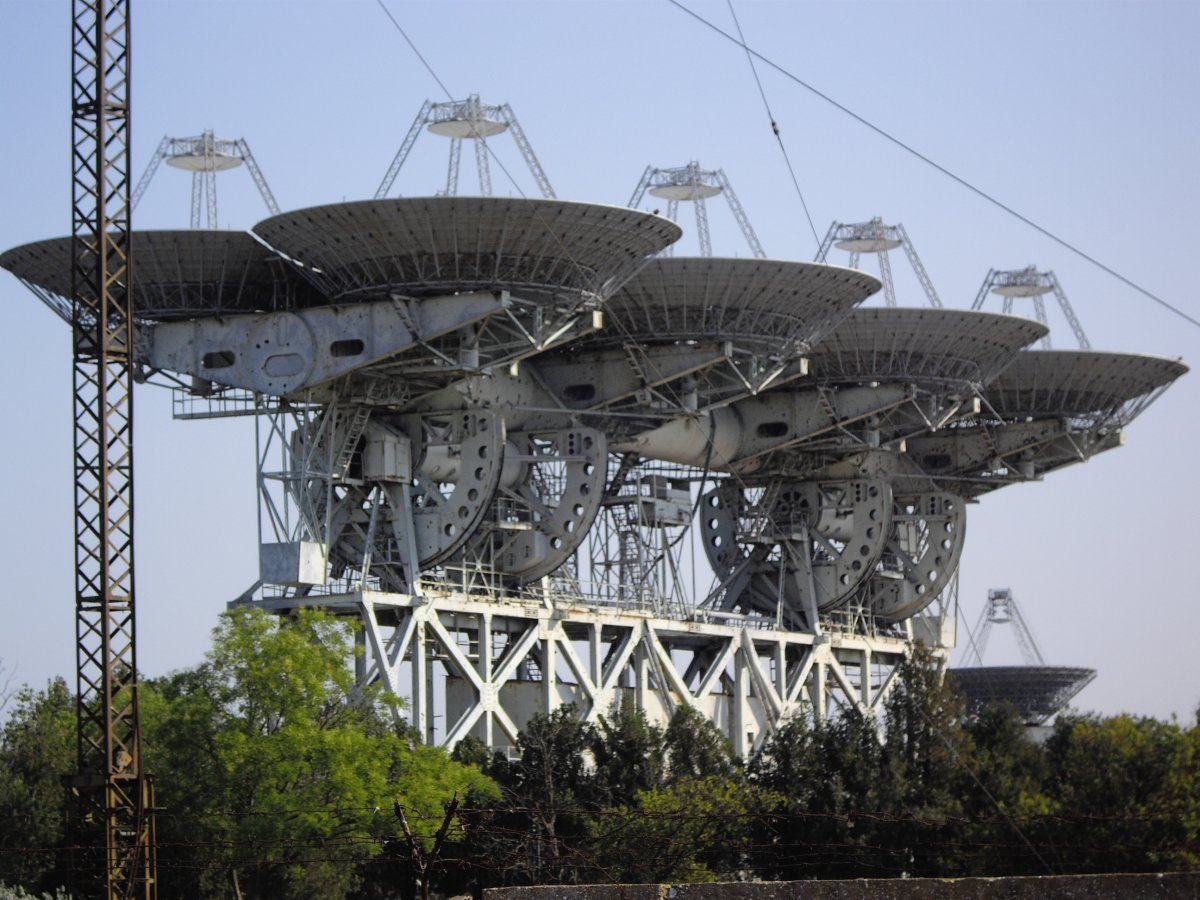
\includegraphics[scale=0.25]{ADU-1000-4.jpg}
  \caption{Pluton radarn, Krim}
  \end{center}
  \label{fig4}
\end{figure}
Tidigare fungerade Areceibo som radar men kabeln som håller mottagaren i brännpunkten brast och det blev
sådan stor skada att den inte kan användas längre.
Radar är inte en framkomlig väg för att mäta stora astronomiska avstånd. Den mottagna
effekttätheten är proportionellt mot $1/r^4$ därför att den reflekterade effekten skall färdas tillbaka
till radarmottagaren och även den effekten sprids ut på en sfärisk yta. För att fördubbla mätavståndet krävs således att radarsändarens uteffekt
ökar med faktorn $2^4 =16$\\

\section{Parallax-mätningar till stjärnor-andra steget}
Spetsen av parallax vinkeln, solen och jorden bildar en rätvinklig triangel där basen $b$ är 1 au och $h$
är avståndet till stjärnan. Låt $p$ vara halva parallax-vinkeln (knappt skönjbar i bilden nedan) då gäller
att
\begin{flalign*}
tan(p) &= \frac{b}{h}\iff\\
h&=\frac{b}{tan(p)}\\
 h &=\frac{ 1\text{ au}}{tan(p)}\\
\end{flalign*}
\begin{figure}[H]
\begin{center}
  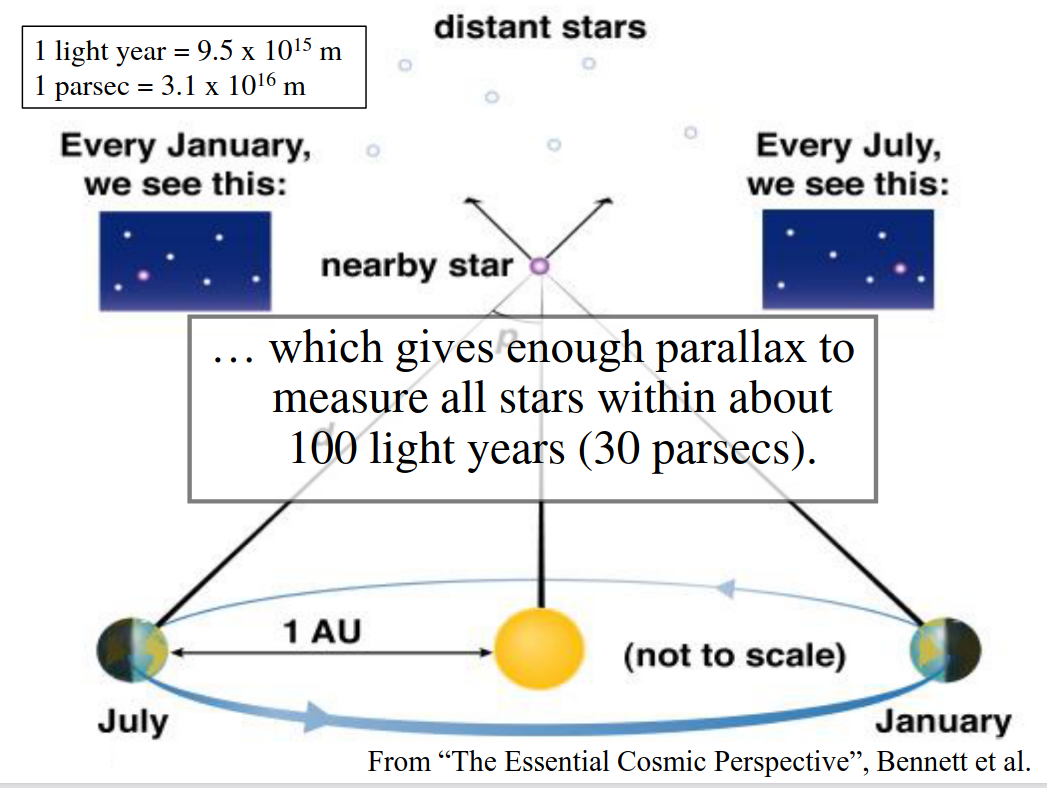
\includegraphics[scale=0.25]{Parallax.png}
  \caption{Parallax mätning}
  \end{center}
  \label{fig4}
\end{figure}
En parsec (pc) definieras som det avståndet vars parallaxvinkel bildar 1 bågsekund då baslinjen är 2 $au$.
\begin{flalign*}
 h\text{ [pc]} &=\frac{ 1\text{ [au]}}{\varphi \text{ [arcsec]}}\\
\end{flalign*}
(Observera att det är halva parallax-vinkeln som ska anges)
Parallaxmätningar gör det möjligt för oss att mäta avståndet till 10 000-tals stjärnor. Det som sätter begränsningen
är atmosfären och instrumentets noggrannhet. Atmosfären bidrar med brytning och spridning av ljuset.
Satelliten Hipparchus (1980-1993) sändes  upp endast för parallaxmätningar. Denna hade en upplösning på
1 millibågsekund och mätte avståndet till ca 100 000 stjärnor upp till 1600 ly (500pc) bort\footnote{\url{https://en.wikipedia.org/wiki/Parallax}}
Satelliten Gaia sändes upp 2013 och beräknas vara verksam till 2025 och används uteslutande till parallaxmätningar.
Dess noggranhet är hela 10 mikrobågsekunder och har därmed förmågan att mäta avstånd på ca 30 000 ly avstånd.
Även Hubble teleskopet används till parallaxmätningar och det har rapporterats om prallaxbestämningar på upp emot
10 000 ly.
Nedan bild visar detektionsgränserna för Gaias, Hipparchus samt gränsen för parallaxmätningar från jorden.
Gaias detektions radie är ringen näst längst till höger (10 000 pc)
från höger till vänster\footnote{\url{https://sci.esa.int/web/gaia/-/27100-gaia-an-ambitious-space-observatory-in-astronomy}}
\begin{figure}[H]
\begin{center}
  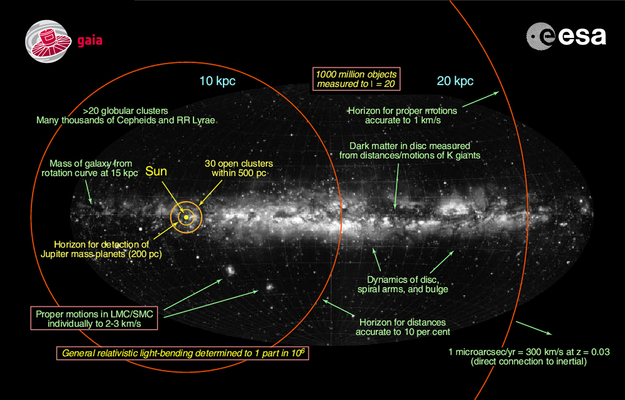
\includegraphics[width=\linewidth]{Gaia.jpg}
  \caption{Detektionsgränser Gaia (10kpc), Hiparchus(500pc) samt jordbaserade parallaxmätningar med avseende på Vintergatan}
  \end{center}
  \label{fig4}
\end{figure}

\section{Spektroskopisk parallax - tredje steget}

Parallax-mätningar har sina uppenbara begränsing vilket är mätinstrumentets noggrannhet. För att komma
längre ut i vintergatan samt till andra galaxer så måste vi ta till statistiska metoder.
Om vi tar de avstånd $r$ som mätts upp med parallaxmätningar och mäter den effekttäthet $F$ (Flux-Watt per kvadratmeter-
Energi per sekund per kvadratmeter) som vår teleskopsensor mäter så kan vi mäta upp den uteffekt $L$ -Luminositet (Watt)
som stjärnan utsänder
\begin{flalign*}
F&=\frac{L}{4\pi r^2}&(1)
\end{flalign*}
faktorn $4\pi r^2$ är arean av en sfär och antagandet är att effekten från stjärnan strålar ut i en sfärisk lobform\footnote{\url{https://en.wikipedia.org/wiki/Inverse-square_law}}
\begin{figure}[H]
\begin{center}
  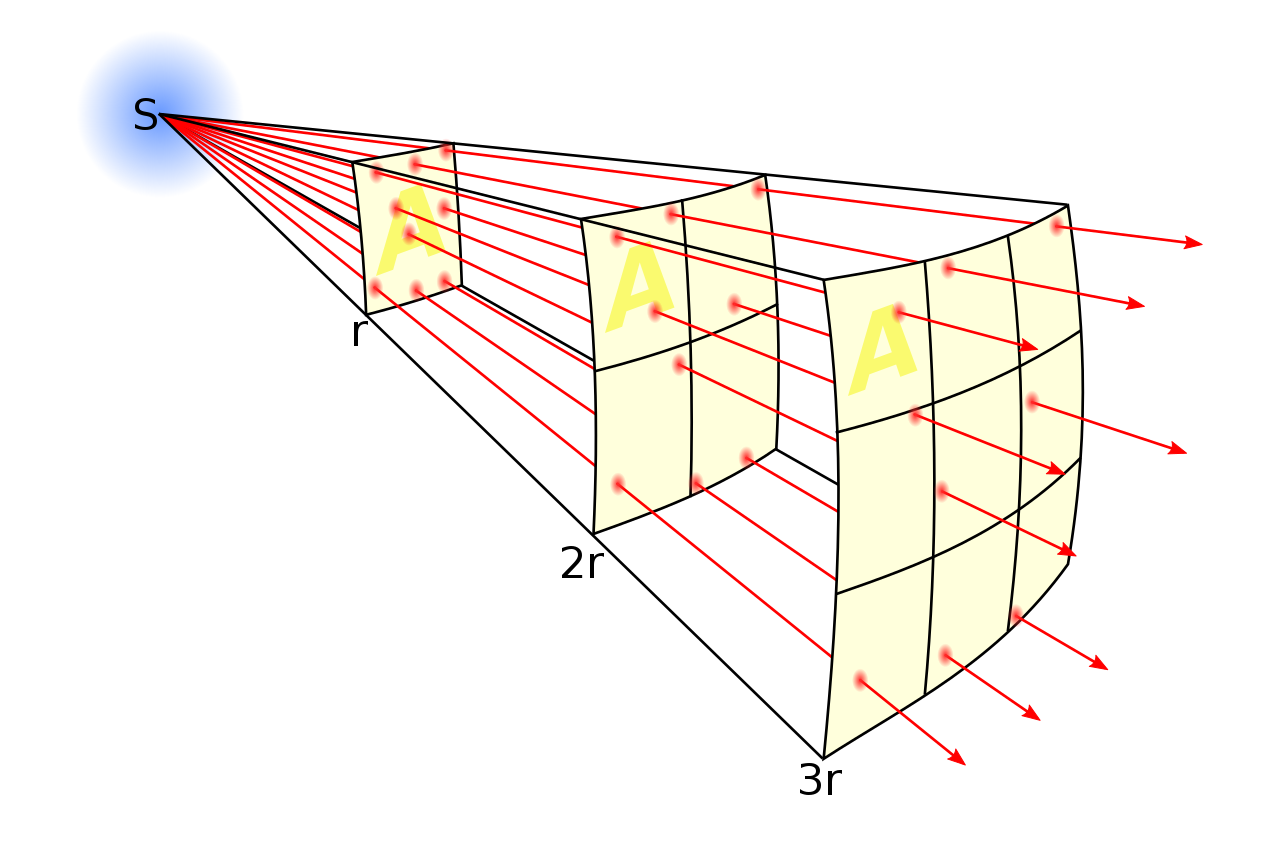
\includegraphics[scale=0.1]{Inverse_square_law.svg.png}
  \caption{Effekttäthet $F$ är uteffekten $L$ dividerad med den klotytan som bildas på avståndet $r$ }
  \end{center}
  \label{fig4}
\end{figure}


Om vi därvid även mäter färgen på stjärnan så kan man plotta färg, uteffekt och effekttäthet vid sensorn
och erhålla ett s.k. Hertzsprung-Russel diagram, ofta förkortat H-R Diagram.
\begin{figure}[H]
\begin{center}
  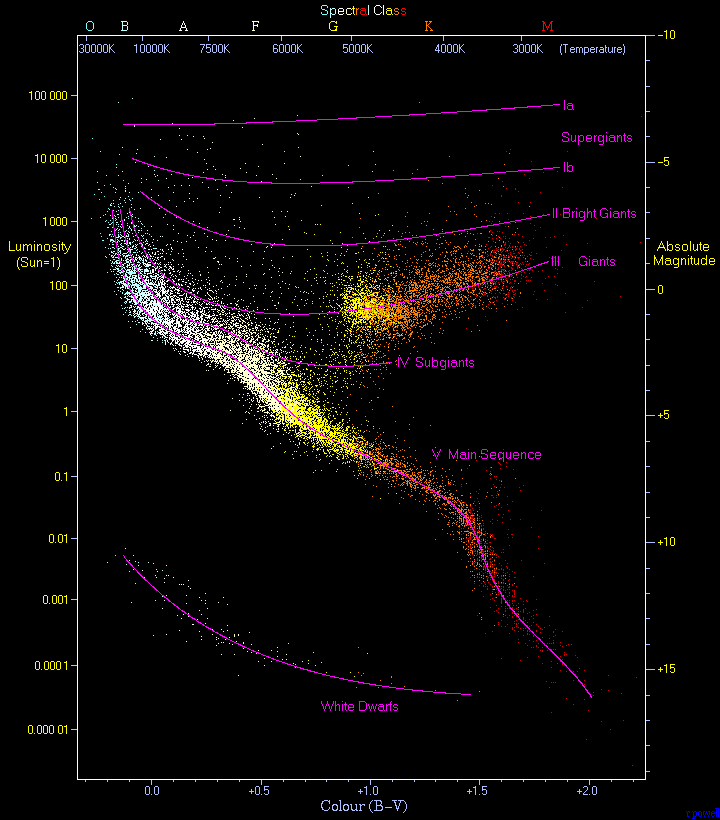
\includegraphics[scale=0.5]{HRDiagram.png}
  \caption{H-R Diagram för 22 000 stjärnor från Hipparchos samt 1000 från Gliese katalogen }
  \end{center}
  \label{fig4}
\end{figure}
Diagrammet listar även temperaturen vilken fås från Wiens förskjutningslag samt den absoluta magnituden vilket
är en alternativ skala till uteffekten $L$ och är härledd från antikens astronomers sätt att ge den ljusstarkaste
stjärnan (de som var först synliga i skymningsljuset) gradtalet 1 och därefter öka siffran till 6 beroende
på hur mycket svagare den uppfattades\footnote{\url{https://en.wikipedia.org/wiki/Apparent_magnitude}}.
Ju mer negativ absolut magnitud desto högre uteffekt och vice versa.

För att beräkna avståndet till en stjärna som ligger för långt bort
för parallaxmätning så tillämpar man den s.k. kosmologiska principen som säger att fördelningen av olika stjärnor i ett volymssampel
av universum innehåller ungefär lika stora mängder olika astronomiska objekt om sampelstorleken är
tillräckligt stor\footnote{\url{https://en.wikipedia.org/wiki/Cosmological_principle}} och därför
anser man att man kan få en rimlig uppfattning om en stjärnas uteffekt (luminositet) genom att
slå upp vad en stjärna med samma färg har för uteffekt i H-R-diagrammet (vars uteffekt man
räknat fram med ekvation $(1)$). Denna princip har dock kritiserat bl.a. av filosofen Karl Popper.
Statistiker menar dock att principen är rimlig dock är det oklart hur stort volymssampel ett tillräckligt stort
volymssampel är, men som en känd tänkare sa \textit{``Man måste börja någonstans''}\footnote{``Skitsamma man måste börja någonstans''-Lasse Karagiannis}\\
Summering av metod
\begin{enumerate}
\item Mät färgen på stjärnan som ligger för långt bort för att parallaxbestämmas
\item Läs av den uteffekt $L$ (eller intervall av uteffekter) färgen motsvara i HR-diagrammet.
\item Mät upp den mottagna effekttäthet $F$ i mätsensensorn $\text{W}/\text{m}^2$
\item Beräkna avståndet enligt
\begin{flalign*}
F&=\frac{L}{4\pi r^2}\iff\\
r&=\sqrt{\frac{L}{4\pi F}}\\
\end{flalign*}
Om intervall av möjlig uteffekt $L$ indikeras av H-R diagrammet (vilket alltid är fallet) relatera
$r_{min}$ till $L_{min}$ och $r_{max}$ till $L_{max}$ och erhåll då med hjälp av formeln på så vis ett intervall av möjliga avstånd $r$ till stjärnan
såsom $r_{min} \leq r \leq r_{max}$\\
Klar!
\end{enumerate}
Problem uppstår för rödaktiga stjärnor därför att H-R diagrammet har två svansar för rött, den övre 
sekvensens av röda jättar sänder på avsevärt högre uteffekt än de röda tillhörande populationen ``main sequence'',
så vad man gör då för att förbättra noggrannheten är att man mäter
avstånd till kluster av stjärnor som ligger förhållandevis nära varandra ca 1 ljusår från varandra och ansätter
ett avstånd $r$ till samtliga stjärnor därför att de sett ur vårt perspektiv ligger alla på ungefär samma
avstånd relativt $r$. Dessa plottas i H-R-diagrammet med förhoppningen att fördelningen skall
se utåsom ``main sequence'' (se diagrammet) med eventuell viss fördelning även hosjättarna och vita dvärgarna.\\

 Om bra överensstämmelse med fördelningen av stjärnor hos
``main sequence'' är fallet så är det enkel sak att öka/minska $r$ så att kurvorna sammanfaller.
Detta kallas ``main sequence fitting'' eller något oegentligt ``spektroskopisk parallax''.
Metoden är rimlig att göra för stjärn-kluster på avstånd upp till ca 10 000 parsec därefter blir det mottagna ljuset från stjärnorna
i stjärnklustret alltför lågt för att kunna urskiljas från varann med de teleskopen vi har på jorden.\\
(10 000 parsec är nästan halva Vintergatan, se figur för Gaias detektionsgräns -ca 10 000 parsec).\\
För att avståndsbedöma till astronomiska objekt ännu längre bort så behövs ljusstarkare objekt än stjärnkluster vilket
kräver ännu en stegpinne på avståndsstegen.\footnote{\url{https://www.youtube.com/watch?v=hP-vN_fteiQ&list=PLEE8A6CB118FADED4&index=4}}


\section{Cepheid variabler -fjärde steget}

På 1700-talet upptäckte astronomer en klass av stjärnor som varierade i ljusstyrka med perioden någon till 
några timmar och dessa är ofta väldigt mycket ljusstarkare då de sänder på sin högsta effekt
En särkilt intressant grupp av dessa variabla stjärnor är gruppen Cepheid variabler.
Dessa utsänder 1000-50 000 gånger högre effekt än solen och har periodtiden
från ca 1 till 50 dagar\footnote{\url{https://youtu.be/iyisAjHdhas?list=PLEE8A6CB118FADED4&t=109}}\\
\begin{figure}[H]
\begin{center}
  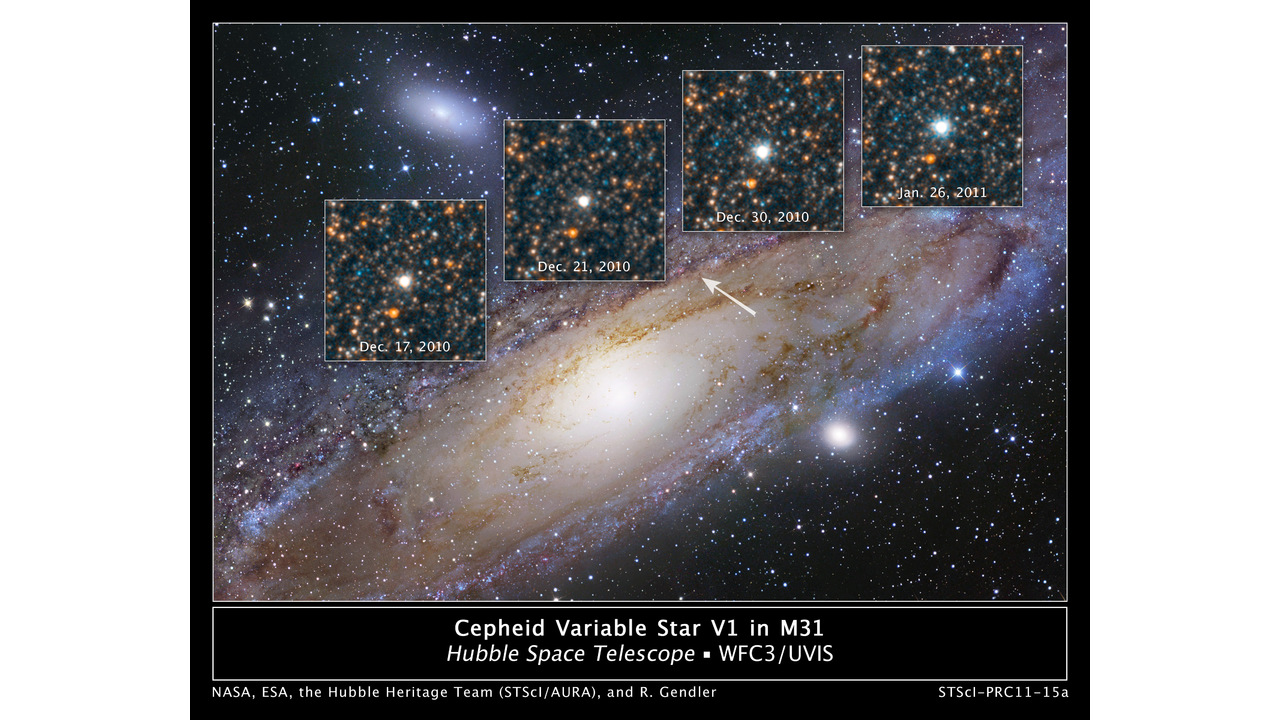
\includegraphics[width=\linewidth]{Cepheid.jpg}
  \caption{Cepheid variabel stjärna i Andromeda galaxen}
  \end{center}
  \label{fig4}
\end{figure}

Astronomen Henrietta Lewitt studerade Stora och lilla Magellanska molnen och upptäckte i början av 1900-talet att de variabla stjärnorna 
har en luminositet som är en funktion av deras periodtid.
Nedan en plott från Leavitts rapport från 1912\footnote{\url{https://articles.adsabs.harvard.edu/pdf/1912HarCi.173....1L}}

\begin{figure}[H]
\begin{center}
  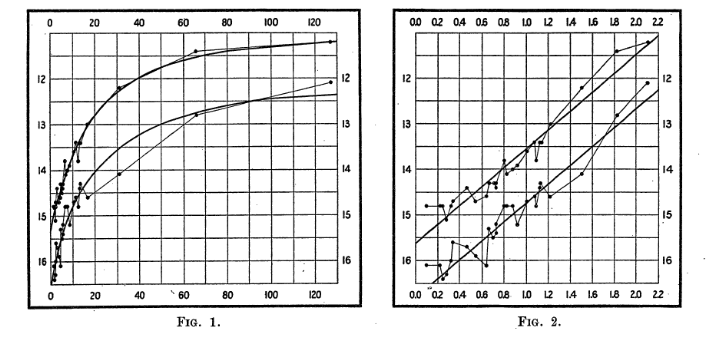
\includegraphics[width=\linewidth]{Henrietta.png}
  \caption{Skenbar magnitud hos 25 Cepheid variabler i Stora magellanska molnet som funktion av dagar (vänster) och som funktion av $\text{log}_{10}(\text{dagar})$ höger -
    Leavitt, Henrietta S.; Pickering, Edward C., 1912 }
  \end{center}
  \label{fig4}
\end{figure}
Det faktum att uteffekt som funktion $\text{log}_{10}(\text{dagar})$ borde rimligen betyda att oscillationerna
beror på samma slags kemiska process och att det därför är ett rimligt antagande att om man återser
en variabel stjärna med samma periodtid så är dess uteffekt densamma som hos den mappade Cepheid variabeln enligt
vanlig logik -\textit{"If it walks like a duck and quacks like a duck it is so because it also most likely that it really is a duck"}.
Hertzsprung kunde dock kort därefter bestämma avståndet till omkringliggande stjärnkluster med hjälp
spektroskopisk parallax s.k. ``main sequence fitting'' användandes av sitt H-R diagram och kunde på så vis
bestämma Cepheid-varibalernas luminositet under antagandet att dessa låg i samma stjärnkluster som stjärnorna
som avståndsbestämningen gjordes till och kunde på så vis plotta en graf med luminositeten som funktion
av periodtiden.Luminositeten som funktion av periodtiden har även vidare kalibrerats med parallaxmätningar.\footnote{\url{https://en.wikipedia.org/wiki/Classical_Cepheid_variable\#Period-luminosity_relation}}

\begin{figure}[H]
\begin{center}
  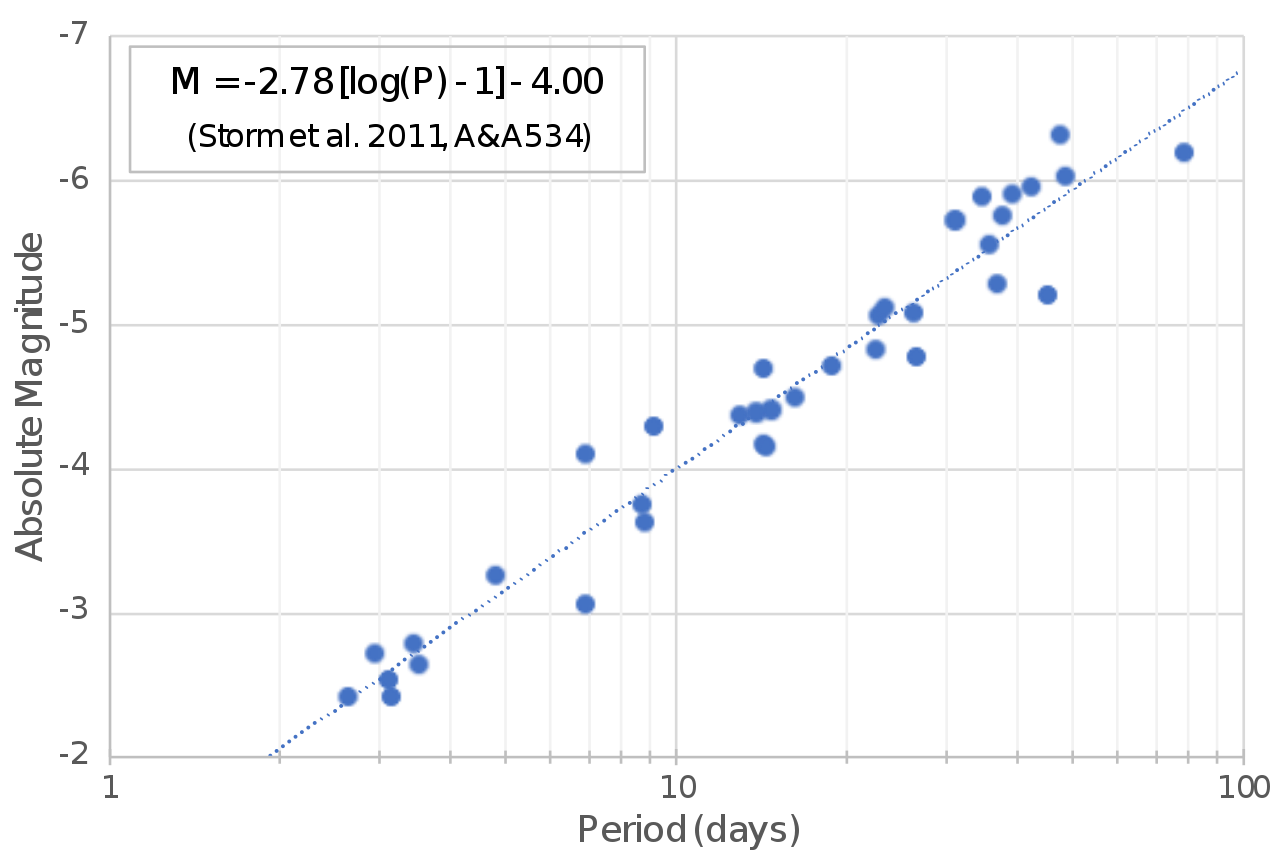
\includegraphics[width=\linewidth]{1280px-Storm2011_Cepheid_Data.svg.png}
  \caption{Absolut Magnitud (relaterar uteffekt P) som funktion av $\text{log}_{10}(\text{dagar})$ hos 35 Cepheidvariabler }
  \end{center}
  \label{fig4}
\end{figure}

Om man således vill mäta avståndet till ett kluster av stjärnor med en närliggande Cepheid variable så
mäter man endast periodtiden och utläser ur grafen dess topp-effekt $L$ med den uppmätta effektätheten $F$
i mätsensorn ger avståndet genom ekvation $(1)$ (som vanligt)
Cepheid variablerna kan användas för att bestämma avstånd upp till 50 Mpc\footnote{\url{https://lco.global/spacebook/distance/cepheid-variable-stars-supernovae-and-distance-measurement/}}
Cepheidvaribalen V1 i Andromeda galaxen har peridotiden 31.4 dagar\footnote{\url{https://youtu.be/iyisAjHdhas?list=PLEE8A6CB118FADED4&t=687}}
Enligt grafen figur 16 så motsvara det Absolut Magnitud $\approx -5.5$. Luminositeten beräknas från formeln\footnote{\url{https://en.wikipedia.org/wiki/Absolute_magnitude\#Bolometric_magnitude}}
\begin{flalign*}
M_{\text{bol}}&=-2.5\text{log}_{10}\frac{L_{star}}{L_0}\iff\\
\frac{M_{\text{bol}}}{-2.5}&=\text{log}_{10}\frac{L_{star}}{L_0}\iff\\
L_{star} &=L_0\cdot 10^{\frac{M_{\text{bol}}}{-2.5}}\\
\end{flalign*}
$L_0=3.0128\times 10^{28}$W är en bolometrisk konstant. Insättning av värden ger
\begin{flalign*}
L_{star} &=3.0128\times 10^{28}\cdot 10^{\frac{-5.5}{-2.5}}\\
         &=4.7750e+30
\end{flalign*}
Effekttäthet uppmätt av Hubbel var enligt youtubekanalen ``PhysicistMicahel''\footnote{\url{https://youtu.be/iyisAjHdhas?list=PLEE8A6CB118FADED4&t=655}}
ca $10^{-15}$ W/$\text{m}^2$. Insatt i formeln $(1)$ ger detta avståndet
\begin{flalign*}
F&=\frac{L}{4\pi r^2}\iff\\
r&=\sqrt{\frac{L}{4\pi F}}\\
 &=\sqrt{\frac{4.7750e+30}{4\pi 10^{-15} }}\\
 &=1.9493\times 10^{22} \text{meter}\\
 &=\frac{1.9493\times 10^{22} \text{ meter}}{9.4605284\times 10^{15} \text{ meter per ly}}=2.0605\text{Mly}
\end{flalign*}
Hubbel fick genomförandes denna räkning $\approx 2.35$Mly men enligt \footnote{\url{https://en.wikipedia.org/wiki/Absolute_magnitude\#Bolometric_magnitude}}
så har sättet att gå från Absolut Magnitud till Luminositet i Watt ändrats så sent som Augusti 2015.
Resultatet visar att Andromeda är en egen galax p.g.a. av avståndet då man tidigare trodde att det var en
stjärn-gas hop i Vintergatan.

Hubbel kalibrerade sin konstant med hjälp av Cepheid variabler och eftersom dess Luminositet-period relation
fortfarande är underlag för ytterliggare kalibrering så rapporteras olika värden på Hubbelkonstanten i litteraturen
från 60km/s/MParsec till 80km/s/Mparsec\footnote{\url{https://en.wikipedia.org/wiki/Classical_Cepheid_variable\#Uncertainties_in_Cepheid_determined_distances}}
Vi kan således hoppa över nästa stegpinne så till vida att vi är tillfreds med kablibreringen Luminocitet - periodtid för Cepheid variablerna.


\section{Typ 1 a Supernovor - femte steget}
Vi behöver en ännu ljustarkare ``standard candle'' för att kunna se längre ut i universum.
Supernovor av typ 1 a uppfyller kriteriet att ha en konsistent luminocitet vilket har
bekräftats med avståndsmätningar till närliggande Cepheid variabler.
Bilden visar att supernovorna beroende på typ kan ha en toppeffekt som är från 30 miljoner till
3 miljarder gånger större än solens vilket låter oss se hundratals miljoner ljusår bort.
\begin{figure}[H]
\begin{center}
  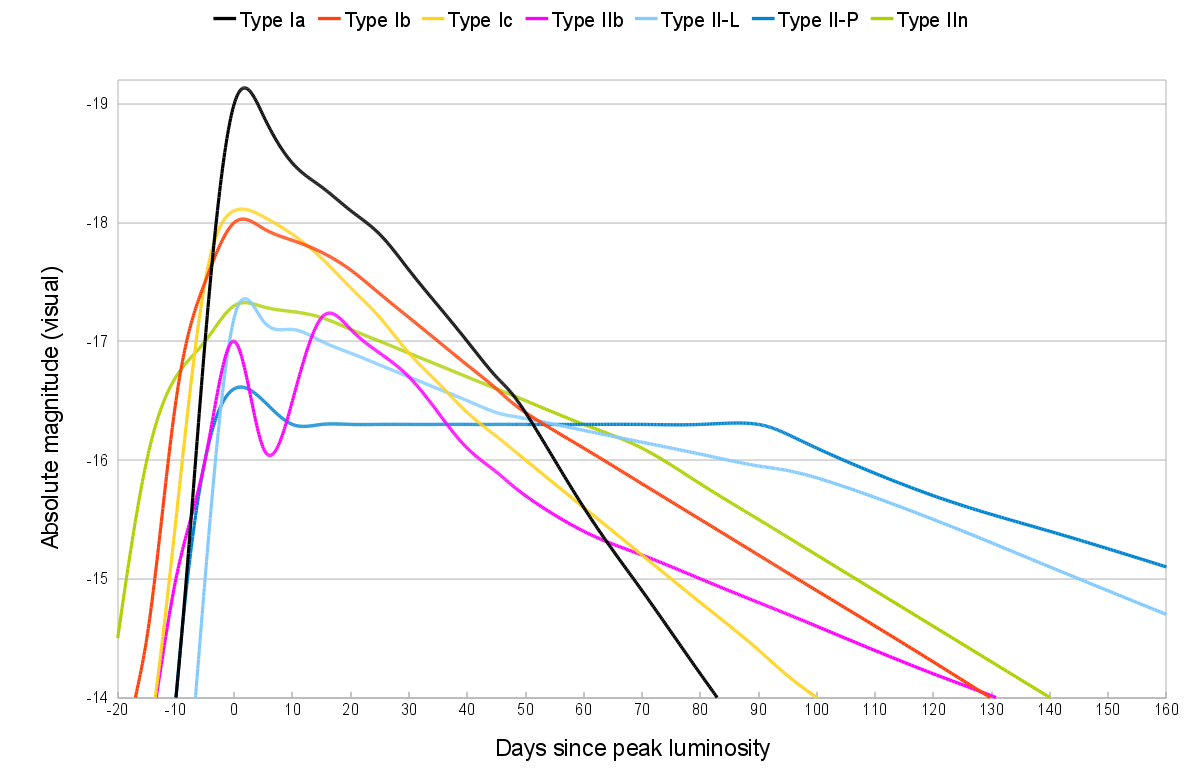
\includegraphics[scale=0.25]{Supernova.png}
  \caption{Absolut magnitud för olika typer av Supernovor }
  \end{center}
  \label{fig4}
\end{figure}

Typ 1 a har varit konsistent i luminicitet varje gång sådan detekteras p.g.a. dess säregna process
varmed den uppkommer. Den uppkommer av att det finns ett stjärnpar nära varandra där den ena stjärnan är en vit dvärg.
Den vita dvärgen rubbar en jämnviktsprocess hos den andra stjärnan i paret när vissa specifika kriterier
är uppfyllda och kommer att suga materia från grannstjärnani en eskalerande kärnreaktion som slutar med en våldsam
smäll där den vita dvärgen slits isär och slungas ut i en våldsam explosion.\\
I Augusti 2011 hände en sådan explosion i Pinnhjulsgalaxen 21 miljoner ljusår bort.
\begin{figure}[H]
\begin{center}
  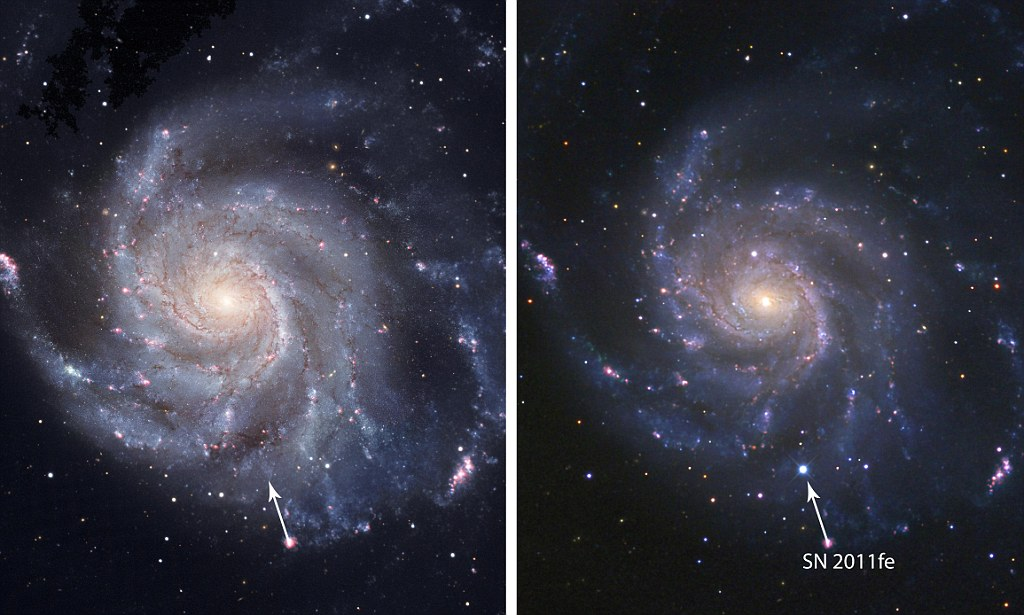
\includegraphics[scale=0.25]{SuperNova_2011fe.jpg}
  \caption{Supernova typ 1a, Pinnhjulsgalaxen ,Augusti }
  \end{center}
  \label{fig4}
\end{figure}
\section{Hubbelkonstanten - sjätte och sista steget}

Den bärande id\'en bakom denna metoden är att ju längre bort en stjärna befinner sig desto längre tid har dess
ljus haft tid på sig att färdas mot observatören på jorden men eftersom universum expanderar så kommer
spektrallinjerna att skiftas mot längre våglängder och ju längre tid som strålningen färdats desto längre tid
har strålningen blivit utsatt för rummets expansion och desto större blir förskjutningen mot längre våglängder
och därmed blir själva våglängsförsljutningen ett mått på hur långt bort stjärnan är.

Grundämnens spektrallinjer uppkommer p.g.a. respektive atoms elektronstruktur, dessa har mätts upp
med spektroskopi men man kan även beräkna dessa på från ren teori ``ab initio'' genom numerisk lösning
av Schrödinger ekvationen med metoder såsom Hartree-Fock och Täthetsfunktionalteori (Density Functional Theory).\\

Ljuset från väteövergångar från avlägsna galaxer vars avstånds bestämts med Cepheid variabler och Supernova
typ 1A har konstaterats att det är alltmer rödförskjutet, vilket betyder att övergångarna synes
translaterade till lägre frekvenser -längre våglängder.
\begin{figure}[H]
\begin{center}
  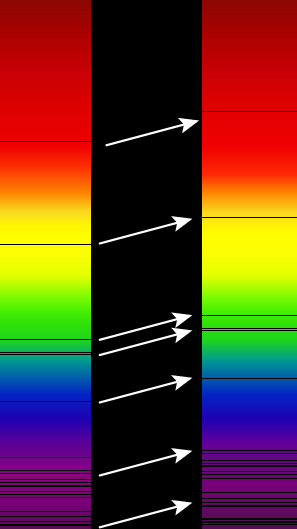
\includegraphics[scale=0.45]{Redshift.png}
  \caption{``Rödskift'' är benämnämningen på fenomenet att grundämnens övergångar blir translaterade till lägre frekvenser }
  \end{center}
  \label{fig4}
\end{figure}

``Rödskiftet'' är alltså en oegentlig benämning därför att det inte avses att ljuset skiftar till rött
eller att endast det röda ljuset skiftas utan man avser att våglängden blir längre än motsvarande
övergång uppmätt i labb för respektive deltagande atom.\\

Rödskiftet betecknas $Z$ och om den uppmätta våglängden betecknas $\lambda$ och dess motsvarande
övergång i ett stillastående labb här på jorden betecknas $\lambda_0$ så definieras
rödskiftet $Z$ såsom den ändringen av väglängden relativt urpsrungsvåglängden 
\begin{flalign*}
Z&=\frac{\lambda - \lambda_0}{\lambda_0}
\end{flalign*}

Man anser att rödskiftet är en linjär funktion av hastigheten hos rummets expansion och/eller objektets
radiella hastighet bort från observatören sådant att 
\begin{flalign*}
Z&=\frac{v}{c}
\end{flalign*}

Hubble relaterade denna hastighet till avståndet $d$ från observatören gånger en konstan $H_0$ - Hubbelkonstanten.
eftersom han upptäckte att objekt som befinner sig på längre avstånd är mer ``rödförskjutna'' dvs. att exempelvis väteövergångar
656 nm blivt förskjuten till allt längre och längre våglängder ju längre bort det astronomiska objekten
befinner sig\footnote{\url{https://en.wikipedia.org/wiki/Hydrogen_spectral_series}}.
\begin{figure}[H]
\begin{center}
  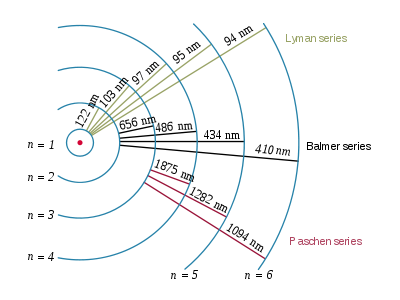
\includegraphics[scale=0.45]{Hydrogen_transitions.svg.png}
  \caption{Några av vätets övergångar uppmätta i labb på jorden }
  \end{center}
  \label{fig4}
\end{figure}

Hubble plottade rödskiftet som funktion av avståndet för den population av galaxer man känner avståndet till
så får man följande graf där $H_0$ är lutningen till den räta linje som bäst minimerar avståndet till varje 
mätpunkt\footnote{\url{https://www.pnas.org/doi/10.1073/pnas.15.3.168}}
\begin{figure}[H]
\begin{center}
  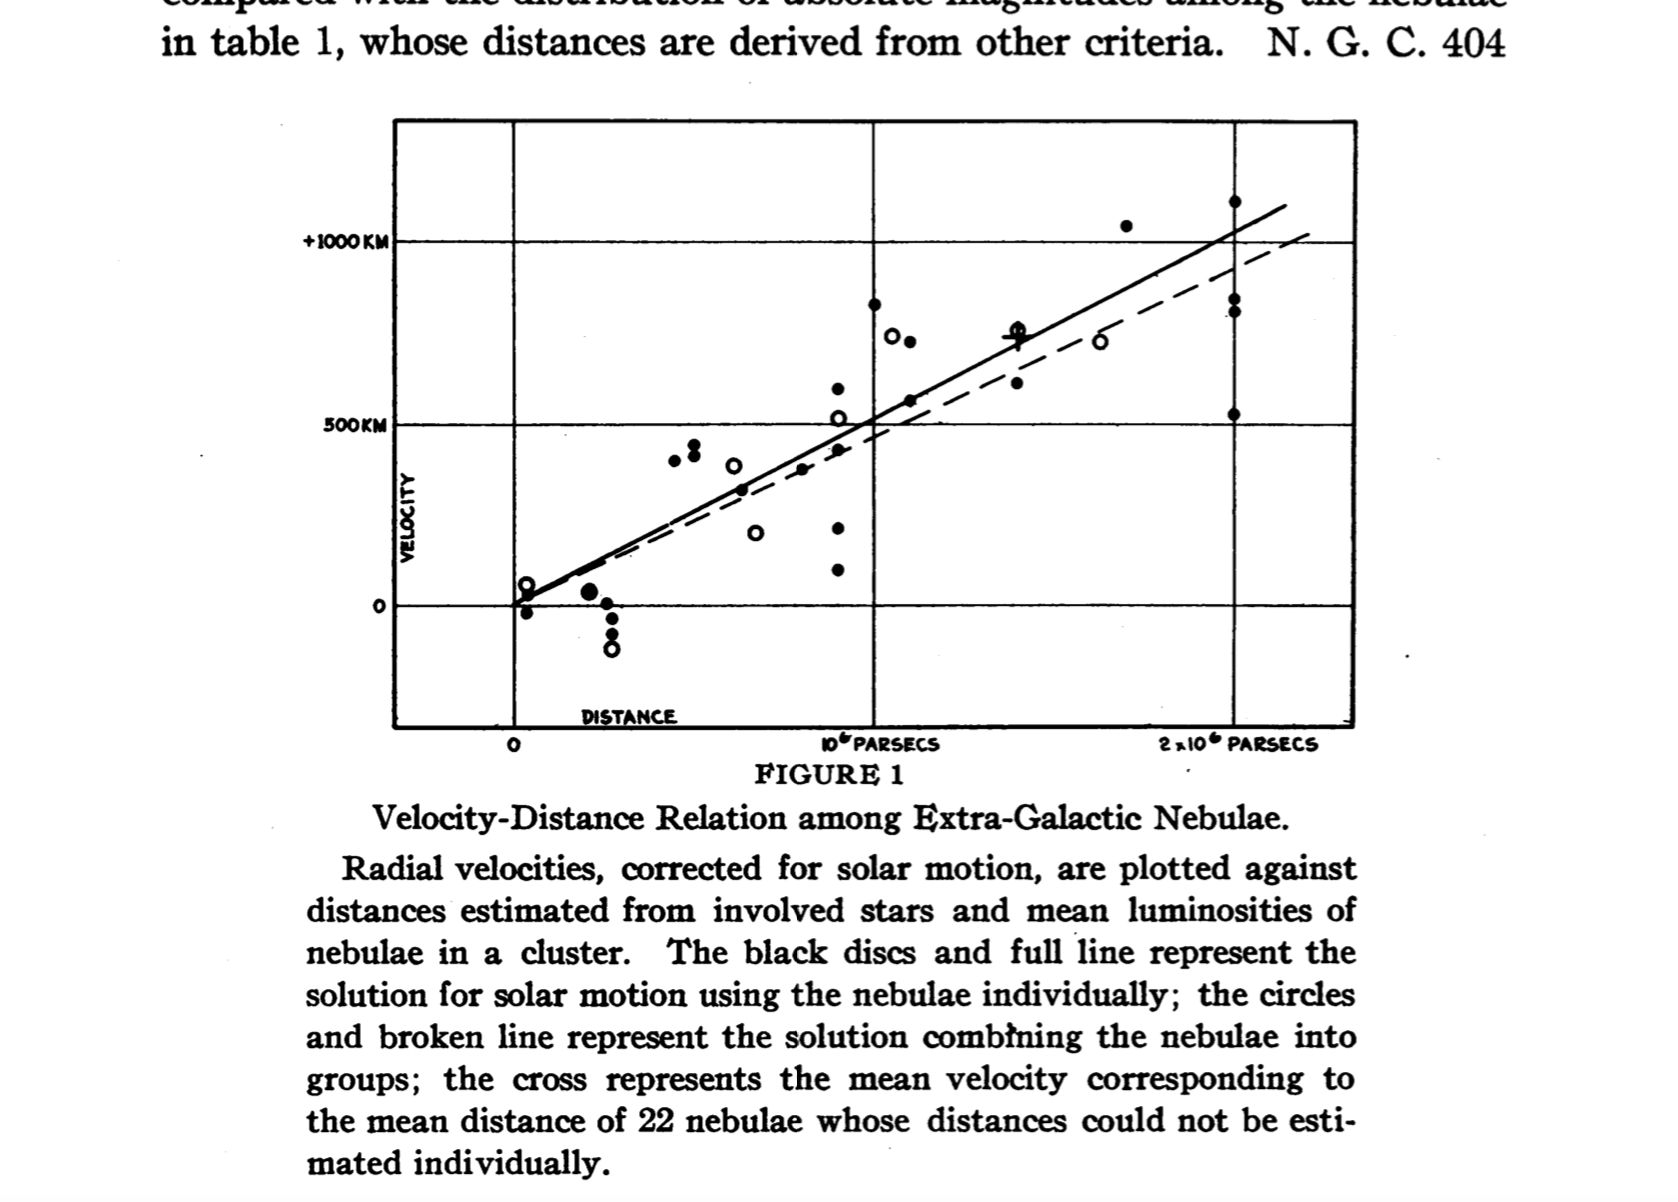
\includegraphics[scale=0.2]{Hubble.png}
  \caption{Hubbles kalibrerade sina avståndsmätningar mot Cepheid variabler }
  \end{center}
  \label{fig4}
\end{figure}

Med korrekt värde på Hubble konstanten så erhålles således den ultimata ``standard candle'' som kan fastställa
avstånd till universums utkanter\footnote{\url{https://physicsanduniverse.com/hubble-law-age-universe/}}

\begin{figure}[H]
\begin{center}
  \includegraphics[scale=0.45]{Hubble-Law-2010.jpeg}
  \caption{Hastigheten $v=c\cdot Z=H_0\cdot d$ }
  \end{center}
  \label{fig4}
\end{figure}


Rödskiftet kan dock ha flera olika orsaker:\\ 
i.) Rummet expanderar och därför dras de elektromagnetiska vågorna ut och blir längre\\
ii.) Objektet har en hastighet bort från observatören, jfr. tonen(frekvensen) från en siren på en uttyckningsbil som är högre
då bilen närmar sig och lägre när den den avlägsnar sig.\\
iii. Enligt Einsteins relativitetsteori så påverkas ljuset av gravitation och då förlorar fotoner
energi då de rör sig från ett objekt med hög gravitation till ett objekt med låg gravitation.
Energin för varje foton är $E=h f=hc/\lambda$, så om energin $E$ minskar så betyder det att våglängden $\lambda$
ökar\footnote{\url{https://en.wikipedia.org/wiki/Gravitational_redshift}}.
\begin{figure}[H]
\begin{center}
  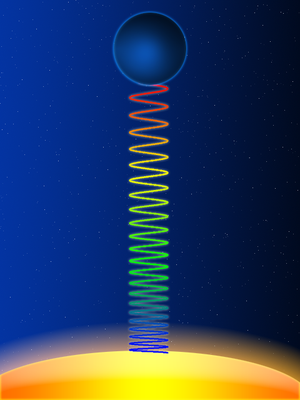
\includegraphics[scale=0.45]{Gravitational_red-shifting2.png}
  \caption{``Rödskift'' p.g.a. att fotoners energi blir lägre då de avgår från ett starkt gravitationsfält till ett svagare gravitations fält. ``Blåskift''- då fotonerna
färdas mot ett starkare gravitationsfält }
  \end{center}
  \label{fig4}
\end{figure}

I runda slängar dock borde det dock vara korrekt att använda metoden.










%\underbrace{}

% \hspace{1em}

%\begin{enumerate}[label=(\alph*)]
%\end{enumerate}

%$$
%  A = 
%  \begin{bmatrix}
%    1 & 0  & 2i\\
%    2i & 0 &  -4\\
%    -i &  0 & -2i\\
%  \end{bmatrix}
%$$

%\begin{flalign*}
%  A = 
%  \begin{bmatrix}
%    1 & 0  & 2i\\
%    2i & 0 &  -4\\
%    -i &  0 & -2i\\
%  \end{bmatrix}
%\end{flalign*}


%\begin{flalign*}
%\psi(x) = \begin{cases} Ae^{ikx}+Be^{-ikx} &\ \  x<-a \\
%                        Ce^{\kappa x}+De^{-\kappa x} &\ \ -a < x < a\\
%						Fe^{ikx} & \ \ x>a
%       \end{cases}
%\end{flalign*}
%[width=80mm,scale=0.7]
%\begin{figure}[H]
%  \includegraphics[width=\linewidth]{odd_finite.eps}
%  \caption{$z_0=0.1\pi,0.5\pi, 3\pi,7\pi$}
%  \label{fig4}
%\end{figure}
\end{document}











                                     
                                     



